\documentclass[10pt,a4paper]{article}

\usepackage[utf8]{inputenc}
\usepackage[T1]{fontenc}
\usepackage[brazil]{babel}
\usepackage{lmodern}
\usepackage[margin=1.8cm,top=1.6cm,bottom=1.6cm]{geometry}
\usepackage{graphicx}
\usepackage{booktabs}
\usepackage{tabularx}
\usepackage{array}
\usepackage{ragged2e}
\usepackage{caption}
\usepackage{enumitem}
\usepackage{amssymb}
\usepackage[hidelinks]{hyperref}
\usepackage{titlesec}

\captionsetup{font=footnotesize,labelfont=bf,skip=2pt}
\setlist{itemsep=0pt,parsep=0pt,topsep=1pt,leftmargin=1.2em}
\renewcommand{\arraystretch}{1.08}
\setlength{\emergencystretch}{2em}
\setlength{\parskip}{2pt}
\setlength{\tabcolsep}{4pt}
\titlespacing*{\section}{0pt}{6pt}{2pt}
\titleformat{\section}{\bfseries\normalsize}{\thesection}{0.5em}{}

\newcolumntype{L}[1]{>{\RaggedRight\arraybackslash}p{#1}}
\newcolumntype{Y}{>{\RaggedRight\arraybackslash}X}
\newcommand{\code}[1]{\texttt{\small #1}}

\pagestyle{empty}

\begin{document}

\begin{center}
{\large\bfseries Monitoramento de um detector de phishing em produção}\\[2pt]
{\small Cibersegurança Aplicada com IA, Insper 2026-2. Roteiro 4, em dupla: Antonio Almeida e Luka Figueiredo.}\\[1pt]
{\footnotesize Notebook com o código, as saídas e os comentários de cada item: \code{roteiro4.ipynb}}
\end{center}
\vspace{1pt}
\hrule
\vspace{5pt}

\noindent
\textbf{Diagnóstico.} O modelo não mudou (o score recalculado bate 100\% com a coluna \code{score}),
mas nas semanas 9 a 40 aconteceram quatro coisas diferentes, cada uma com causa e resposta próprias:
(1) \textbf{drift de dados} súbito nas semanas 13--16, que virou falso positivo;
(2) \textbf{envenenamento pelo feedback}: 8 caixas passam a liberar phishing da quarentena a partir da semana 18, de forma gradual;
(3) \textbf{quebra de pipeline} nas semanas 22--25 (\code{idade\_dominio\_dias} $=0$ em 50\% dos e-mails);
(4) \textbf{drift de conceito} a partir da semana 30: fraude de pagamento com cara de e-mail legítimo derruba o recall de 0,95 para $\approx$0,5.
O retreino automático com \code{rotulo\_pipeline} \textbf{não deve ser ligado}: piora o detector e é exatamente o canal do ataque.

\begin{figure}[h]
\centering
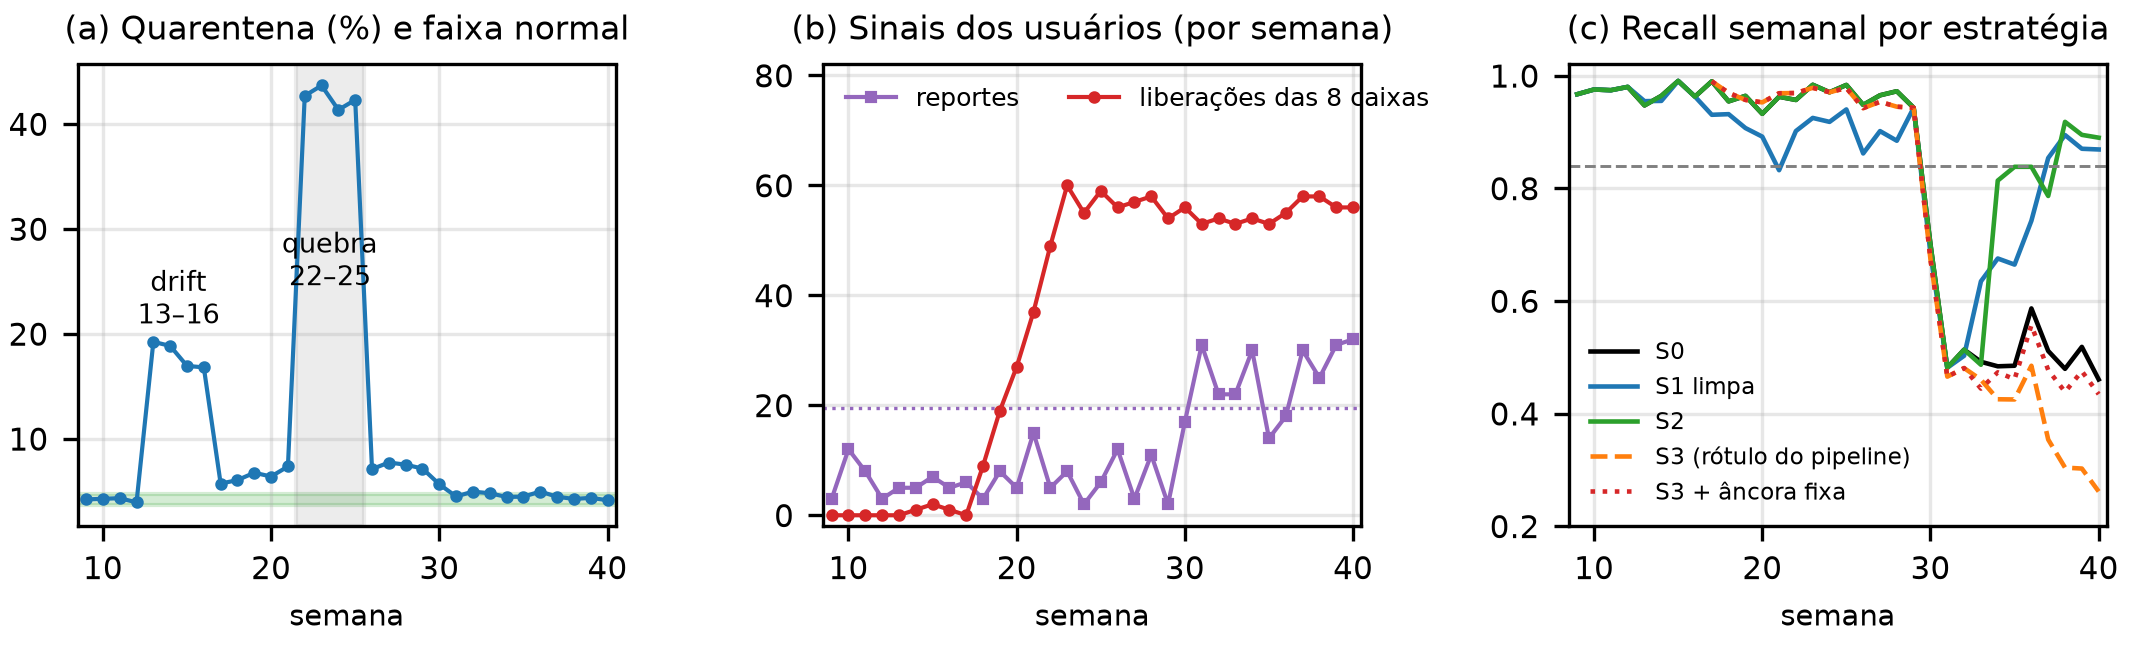
\includegraphics[width=\textwidth]{fig_relatorio.png}
\caption{(a) Fração em quarentena com a faixa normal (semanas 9--12). (b) Reportes (linha pontilhada: limite superior da faixa) e liberações vindas das 8 caixas suspeitas. (c) Recall semanal com o rótulo verificado; tracejado cinza: recall de base $-$ 0,15.}
\end{figure}
\vspace{-8pt}

\section*{a) Linha de base e painel sem rótulos}
Nas semanas 7 e 8, com limiar 0,30, a precisão é 0,883 e 0,942 (média \textbf{0,913}) e o recall 0,990 e 0,991 (média \textbf{0,991}).
A faixa normal (média $\pm$ 3 desvios amostrais das semanas 9--12) é 3,7--4,7\% de quarentena, 0,032--0,045 de score médio, 4,6--12,4 liberações e até 19,6 reportes por semana.
O painel sai da faixa em quatro períodos.
\textbf{13--16}: quarentena em 17--19\% e liberações $\times$17, espalhadas ($\approx$1 por caixa), com reportes normais. O modelo está retendo e-mail legítimo.
\textbf{17--21 e 26--30}: quarentena de 6--8\% e liberações de 27 a 87 por semana, vindas de só $\approx$30 caixas.
\textbf{22--25}: degrau para 41--44\% de quarentena e $\approx$460 liberações, com início e fim abruptos, o que sugere uma falha de pipeline.
\textbf{31--40}: quarentena e score \emph{voltam} à faixa, mas os reportes sobem para 22--32 por semana, sinal de phishing chegando na caixa de entrada. E metade da quarentena é liberada por $\approx$25 caixas (taxa de liberação de 50\%, contra 7\% na base).

\section*{b) Qualidade dos dados}
Não há nulos, e as binárias mantêm dois valores. Uma única feature quebra: \code{idade\_dominio\_dias} vale \textbf{0 em 50,0\% dos e-mails das semanas 22--25}, um valor que não existe na referência (mínimo de 1 dia). A fração fora da faixa vai de 0 a 0,50, e o número de distintos cai de $\approx$1.400 para $\approx$780.
\textbf{Efeito:} nessas semanas os e-mails com idade 0 vão 78\% para a quarentena, contra 7\% dos intactos, com a mesma prevalência de phishing (5,9\% e 5,5\%). São $\approx$\textbf{4.400 quarentenas a mais} e 1.689 das 1.831 liberações do período. Zerar a feature em semanas sãs leva a quarentena de 7\% para 77\%.
\textbf{Não é drift}: os e-mails são os mesmos, o que mudou foi a medição. \textbf{Pipeline:} tratar a falha do WHOIS como ausente (nunca 0), validar o esquema na entrada e reprocessar a quarentena afetada. \textbf{Retreino:} as semanas 22--25 ficam fora de qualquer janela, ou o modelo aprende o defeito.

\section*{c) Drift de dados}
\textbf{1.} PSI $\geq$ 0,10 só em dois episódios. Nas \textbf{semanas 13--16}: \code{idade\_dominio\_dias} (0,13--0,18), \code{link\_divergente} (0,11--0,16), \code{pede\_credencial} (semanas 13--14) e \code{primeiro\_contato} (semana 13), além do \code{score} (0,14--0,18). É um drift súbito e temporário: chegou e-mail com domínios mais novos, mais links divergentes e mais pedidos de login (\code{pede\_credencial}: 0,06 $\to$ 0,16). Nas \textbf{semanas 22--25} o PSI de 1,1--1,2 em \code{idade\_dominio\_dias} e \code{score} é a quebra do item b), não drift.
\textbf{2.} \code{tamanho\_kb} tem KS com $p<0{,}01$ em \textbf{28 das 32 semanas}, mas PSI máximo de 0,078. A mediana sobe devagar de 50 para 61~KB, a feature tem importância de 0,05 e a quarentena não se mexe. Com milhares de linhas, o KS acusa diferenças minúsculas, e 416 testes geram $\approx$4 alarmes por acaso. Significância não é relevância.
\textbf{3.} A \textbf{subida dos reportes nas semanas 31--40} não aparece: nesse período nenhuma feature passa de PSI 0,078, e o PSI do score fica abaixo de 0,01. Também não aparecem as liberações concentradas, que são comportamento dos usuários, nem a mudança de prevalência (de 3,8\% para $\approx$6\%), escondida na classe rara.

\section*{d) Drift de conceito}
O recall fica entre 0,93 e 0,99 até a semana 29; o drift e a quebra derrubam a \emph{precisão}, não o recall. Na \textbf{semana 30} o recall cai para \textbf{0,701}, abaixo de $0{,}991-0{,}15=0{,}841$, e depois fica em 0,46--0,59. Pela tabela do que se sabia ($t-3$), a queda só é \textbf{conhecida no início da semana 33}.
O \textbf{Page-Hinkley} fica em silêncio até a semana 29 e dispara na \textbf{semana 30}, no 16º phishing daquela semana. Como o fluxo depende do rótulo, o alarme também só existe no início da semana 33.
O primeiro sinal sem rótulo, os reportes acima da faixa na \textbf{semana 31}, é conhecido no início da 32: \textbf{uma semana antes}.
O PSI não acusou porque a mudança está \emph{dentro} do phishing: calculado só sobre o phishing, ele chega a 3,6 (\code{n\_links}) e 1,3 (\code{idade\_dominio\_dias}), mas no tráfego todo fica abaixo de 0,06. Os phishing perdidos têm domínio antigo, SPF/DKIM ok, quase nenhum link e não pedem senha, mas 84\% \textbf{pedem pagamento}, feature com importância $\approx$0 no modelo. Mudou $P(y\mid X)$ numa classe de $\approx$6\% do tráfego, e o PSI só olha $P(X)$.

\section*{e) Estratégias de retreino}
\begin{center}
\footnotesize
\begin{tabular}{lcccc}
\toprule
 & precisão 26--29 & precisão 30--40 & recall 30--40 & retreinos \\
\midrule
S0 (estático) & 0,752 & 0,652 & 0,519 & 0 \\
S1 (a cada 4 semanas) & 0,886 & 0,792 & 0,696 & 7 \\
S1 limpa (sem 22--25) & \textbf{0,894} & 0,790 & 0,716 & 7 \\
S2 (gatilho: reportes; sem. 32, 34, 38, 40) & 0,752 & 0,767 & \textbf{0,742} & \textbf{4} \\
\bottomrule
\end{tabular}
\end{center}
\vspace{-3pt}
O atraso do rótulo decide o resultado. Como o rótulo da semana 30 só chega na 33, o retreino da S2 na semana 32 ainda não vê a campanha, mas o da 34 (com 2 semanas de campanha) leva o recall a 0,81. A S1, presa ao calendário, só se recupera na 37.
A S1 parece melhor na semana 25 (precisão 0,87 contra 0,11) só porque \textbf{aprendeu o defeito} (``idade 0 = legítimo''), uma regra que um atacante pode explorar. A S1 limpa é a forma correta.
\textbf{Recomendação: S2}, com dois ajustes. O phishing que passa é fraude de pagamento, cujo custo supera o de um falso positivo, então o recall pesa mais. E ela faz 4 retreinos contra 7, com menos rotulagem e validação. Como o gatilho só por reportes ignora a precisão (0,752 nas semanas 26--29), acrescento um gatilho por quarentena fora da faixa (com rearme da faixa e só após a checagem de qualidade) e a priorização da rotulagem pelo SOC quando um gatilho disparar.

\section*{f) Feedback, envenenamento e portão}
\textbf{1.} Na S3, o recall no ouro cai devagar e sem parar, de \textbf{0,976} (semana 17) para \textbf{0,820} (semana 40), no máximo $-$0,033 por semana. A precisão no ouro fica em $\approx$0,99, e o recall real termina em \textbf{0,26}, pior que o do modelo estático (0,46).
\textbf{2.} O \textbf{portão relativo não bloqueia nenhuma semana}, porque o limite desce junto (de 0,939 para 0,778); o recall médio real nas semanas 30--40 é 0,422. A \textbf{âncora fixa bloqueia nas semanas 33--40} (candidato 33: 0,9375 $<$ 0,9392) e congela o candidato 32, com recall médio real de 0,489. Ela impede o modelo de esquecer, mas não o faz aprender a campanha nova, que não está no ouro.
\textbf{3.} Nas semanas 18--40, \textbf{8 caixas (0,27\%) respondem por 36,5\% das liberações} (1.146 de 3.141; a 9ª caixa tem 5), e \textbf{99,7\%} do que liberam é phishing verificado, contra 2,6\% nas demais. O volume cresce aos poucos (9, 19, 27, 37, 49, 60 por semana) e depois se estabiliza em $\approx$55.
\textbf{4.} Dos 948 phishing que passaram nas semanas 30--40, só \textbf{20,7\%} são 1 no \code{rotulo\_pipeline}; os outros 79,3\% entram no treino como legítimos.
\textbf{Conclusão:} não ligar o retreino com o rótulo do pipeline. Ele combina cegueira, ciclo de realimentação e um \textbf{sapo na panela} real: o veneno entra aos poucos, cada retreino perde menos que a tolerância, e o portão relativo desce junto. Para ligar algum retreino é preciso: rótulo verificado; peso limitado por caixa no feedback; âncora fixa no ouro, com o ouro ampliado pelo SOC com ataques novos; exclusão de semanas quebradas; e aprovação humana.

\section*{g) Plano de monitoramento e automação}
\begin{center}
\scriptsize
\begin{tabularx}{\textwidth}{@{}L{2.0cm}L{3.5cm}L{3.1cm}L{2.1cm}Y@{}}
\toprule
\textbf{Sinal} & \textbf{Como medir} & \textbf{Limiar de alarme} & \textbf{Quem} & \textbf{Primeira ação} \\
\midrule
1. Qualidade dos dados & Por feature/semana: nulos, zeros, distintos, fração fora de [mín,máx] da referência & Fora da faixa $>$1\%; zeros/nulos variando $>$0,20; distintos $<$60\% & Eng. de dados (gateway) & Checar o extrator; tratar como ausente e imputar; marcar a semana ``fora do treino'' \\
2. Drift de dados & PSI por feature e do score $\times$ referência; KS só como contexto & PSI $\geq$0,10 atenção, $\geq$0,25 ação (após descartar o sinal 1) & Dono do modelo & Ver o segmento novo e o efeito na quarentena; amostra rotulada pelo SOC \\
3. Saída do modelo & Fração em quarentena e score médio, diário e semanal & Fora de média $\pm$3 desvios da base (refeita a cada troca de modelo) & Plantão SOC + dono do modelo & Cruzar com 1, 2 e 4 (FP $\times$ phishing passando); amostrar a quarentena \\
4. Reportes & Reportes ($+1$) por semana e o conteúdo deles & $>$ limite superior da faixa ($\approx$19,6) & SOC (incidente) & Achar a campanha; priorizar rotulagem; regra temporária (pedido de pagamento externo) \\
5. Concentração das liberações & Liberações ($-1$) por caixa e semana & $\geq$3 caixas com $\geq$3 liberações na semana (base: nenhuma) & Segurança/SOC + dono do modelo & Tirar o feedback dessas caixas do treino; verificar o que liberaram; investigar as contas \\
6. Desempenho com rótulo & Precisão/recall semanais ($t-3$); Page-Hinkley no fluxo de phishing perdido & Recall $<$0,841; precisão $<$0,81; disparo do PH & Dono do modelo + gestor do SOC & Analisar os erros; retreino com rótulo verificado (janela limpa) \\
7. Integridade do retreino & Candidato no ouro $\times$ âncora fixa; $\times$ modelo atual no tráfego recente; origem dos rótulos & Recall no ouro $<$0,939; pior que o atual; janela com semana marcada ou caixa do sinal 5 & Dono do modelo + aprovador humano & Bloquear a promoção; manter o modelo; revisar a janela \\
8. Fidelidade do rótulo automático & Fração dos phishing verificados com \texttt{rotulo\_pipeline}\,$=1$ & $<$0,80 & Dono do modelo & Proibir esse rótulo no treino \\
\bottomrule
\end{tabularx}
\end{center}
\vspace{-3pt}
\textbf{Replay no histórico:} o sinal 3 acusa o drift no início da semana 14, o 1 acusa a quebra na 23, o \textbf{5 acusa o envenenamento na 20}
(13 semanas antes de o rótulo mostrar a queda de recall), o 4 acusa o drift de conceito na 32 e o 7 bloqueia a S3 na 33.
\textbf{Frameworks.} \textbf{AML.T0020} (Training Data Poisoning) é o ataque pelo feedback; os sinais 5, 7 e 8 são a defesa, e treinar só com rótulo verificado fecha o canal.
\textbf{AML.T0031} (Erode AI Model Integrity) explica por que o portão usa âncora fixa.
\textbf{AML.M0008} (Validate AI Model) é o sinal 7, junto com a validação contínua dos sinais 2, 3 e 6; drift e envenenamento são investigados juntos.
\textbf{NIST MEASURE 2.4}: sinais 1--6 e 8 monitoram o comportamento em produção.
\textbf{NIST MANAGE 4.1}: os sinais 4--5 captam e auditam a contribuição dos usuários, as colunas ``quem'' e ``primeira ação'' formam a resposta a incidentes, o rollback é a recuperação e o portão com aprovação é a gestão de mudanças.

\textbf{Automação.} O pipeline pode, \emph{sem aprovação}: calcular os sinais e abrir alarmes; marcar semanas com falha de qualidade; treinar candidatos só com o rótulo verificado pelo SOC (janela $t-10$ a $t-3$, sem semanas marcadas nem feedback de caixas sinalizadas); avaliá-los no ouro e no tráfego recente; e voltar ao último modelo aprovado se um sinal de desempenho disparar. \emph{Precisa passar pelo portão e por uma pessoa} tudo o que muda o que o modelo aprende ou o que conta como verdade: promover um candidato (âncora fixa no ouro, não ser pior que o atual e aprovação do dono do modelo), mudar o limiar, a âncora ou o ouro (que só cresce com exemplos verificados) e usar qualquer rótulo não verificado. Esse desenho \textbf{impede o envenenamento gradual pelo feedback} (sapo na panela) encontrado no item f). As liberações das 8 caixas não viram rótulo; mesmo que virassem, o sinal 5 dispararia na semana 19, a âncora fixa não desce com o modelo e nenhuma troca de modelo ocorre sem revisão humana.

\end{document}
